\documentclass[12pt,a4paper]{article}
\usepackage{graphicx}
\graphicspath{{images/}}
\usepackage{hyperref}
\usepackage{geometry}
\geometry{margin=2cm}
\usepackage{xcolor}
\usepackage{float}
\usepackage{booktabs}
\usepackage{enumitem}
\usepackage{xepersian}
\settextfont{Tahoma}

\title{\textbf{راهنمای جامع کاربری و تصویری گام به گام nopCommerce}\\
\large(صفحه تخفیف‌های شگفت‌انگیز، سیستم تبلیغات فروشندگان، خرید گروهی و کیف پول)}
\author{مستندات توسعه و کاربری سیستم nopCommerce فارسی}
\date{\today}

\begin{document}

\maketitle
\tableofcontents
\newpage

\section{مقدمه و آدرس برنامه}
این راهنما جهت استفاده کاربران نهایی (مشتریان)، فروشندگان (تامین‌کنندگان) و مدیران فروشگاه nopCommerce به زبان فارسی تنظیم شده است. تمامی مراحل به همراه تصویر مربوط به آن گام به گام ارائه گردیده است.

\begin{center}
\textbf{آدرس آنلاین فروشگاه:} \url{https://ground-buggy-karaoke.ngrok-free.dev}
\end{center}

\begin{figure}[H]
    \centering
    \setlatin{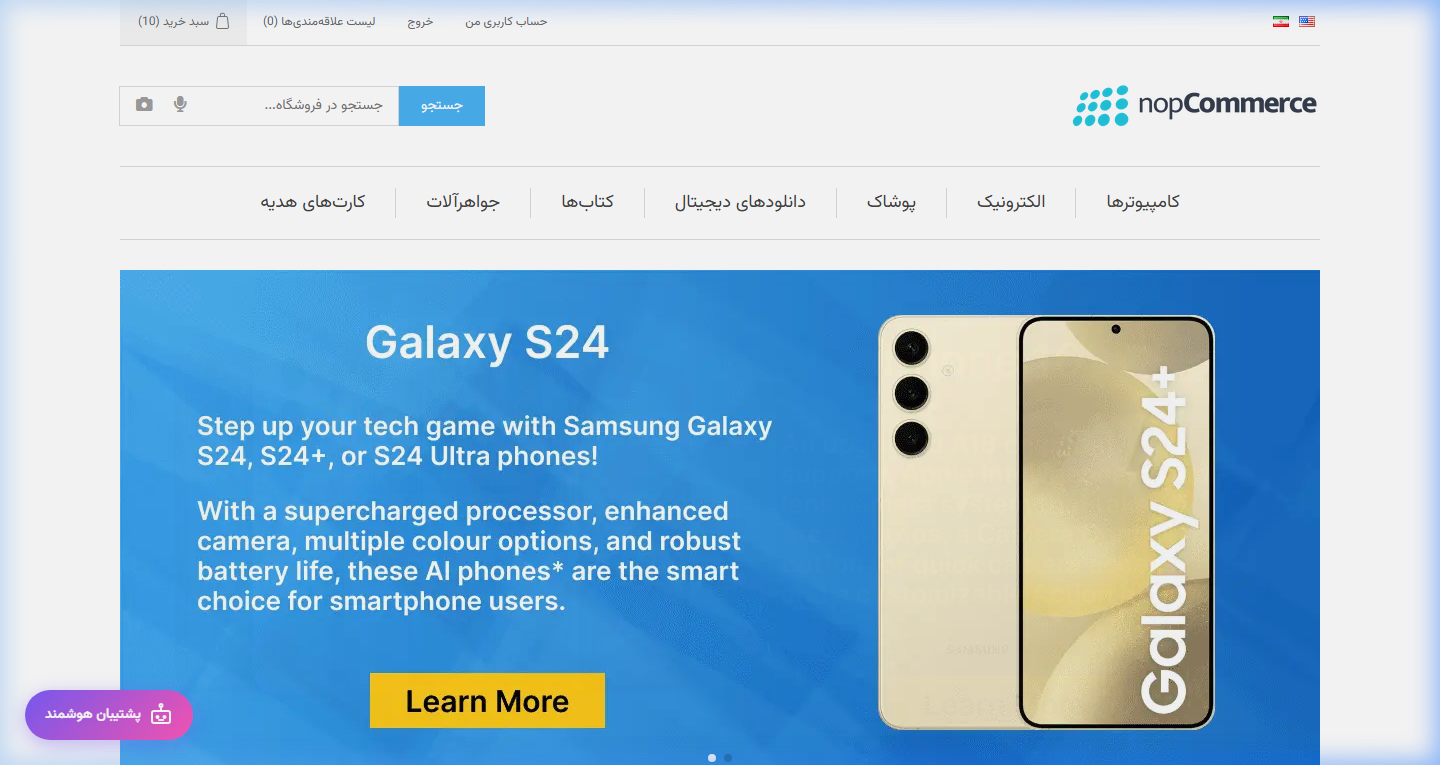
\includegraphics[width=0.85\textwidth]{persian_home.png}}
    \caption{نمای کلی صفحه اصلی فروشگاه با زبان فارسی و راست‌چین (RTL)}
    \label{fig:persian_home}
\end{figure}

\section{معرفی ماژول‌های هوشمند سیستم}
سیستم پیشرفته nopCommerce به ماژول‌های هوشمند زیر مجهز گردیده است:
\begin{itemize}[label=\small$\bullet$]
    \item \textbf{ماژول B (جستجوی هوشمند):} جستجوی صوتی و تصویری هوش مصنوعی (نسخه ابری/محلی).
    \item \textbf{ماژول C (تشخیص محصولات تکراری):} تشخیص محصولات تکراری با هوش مصنوعی جهت جلوگیری از ثبت تکراری کالاها در پنل انبارداری.
\end{itemize}

\section{پیش‌نیازهای سیستم و تنظیمات فونت فارسی}
برای کارکرد صحیح افزونه‌ها و نمایش کامل زبان فارسی:
\begin{enumerate}
    \item \textbf{تنظیم زبان اصلی:} در پنل مدیریت به مسیر \lr{Configuration > Languages} مراجعه نموده و زبان فارسی (\lr{fa-IR}) را فعال و به عنوان زبان پیش‌فرض انتخاب کنید.
    \item \textbf{بومی‌سازی و قلم وزیرمتن:} تمامی بخش‌های افزونه‌ها به ترجمه کامل فارسی مجهز شده و از قلم استاندارد **Vazirmatn** استفاده می‌کنند.
\end{enumerate}

\newpage
\section{بخش اول: راهنمای گام به گام صفحه تخفیف‌های شگفت‌انگیز}

صفحه تخفیف‌های شگفت‌انگیز تمامی کالاهای دارای تخفیف فعال را در یک ویترین یکپارچه نمایش می‌دهد.

\subsection{گام ۱: نحوه تعریف تخفیف شگفت‌انگیز توسط مدیر (Admin)}
وارد پنل مدیریت شوید و به مسیر \textbf{ترفیعات > تخفیف‌ها} (\lr{Promotions > Discounts}) بروید. تخفیف جدید با نوع \lr{Assigned to products} ایجاد کنید و درصد تخفیف را وارد نمایید.

\begin{figure}[H]
    \centering
    \setlatin{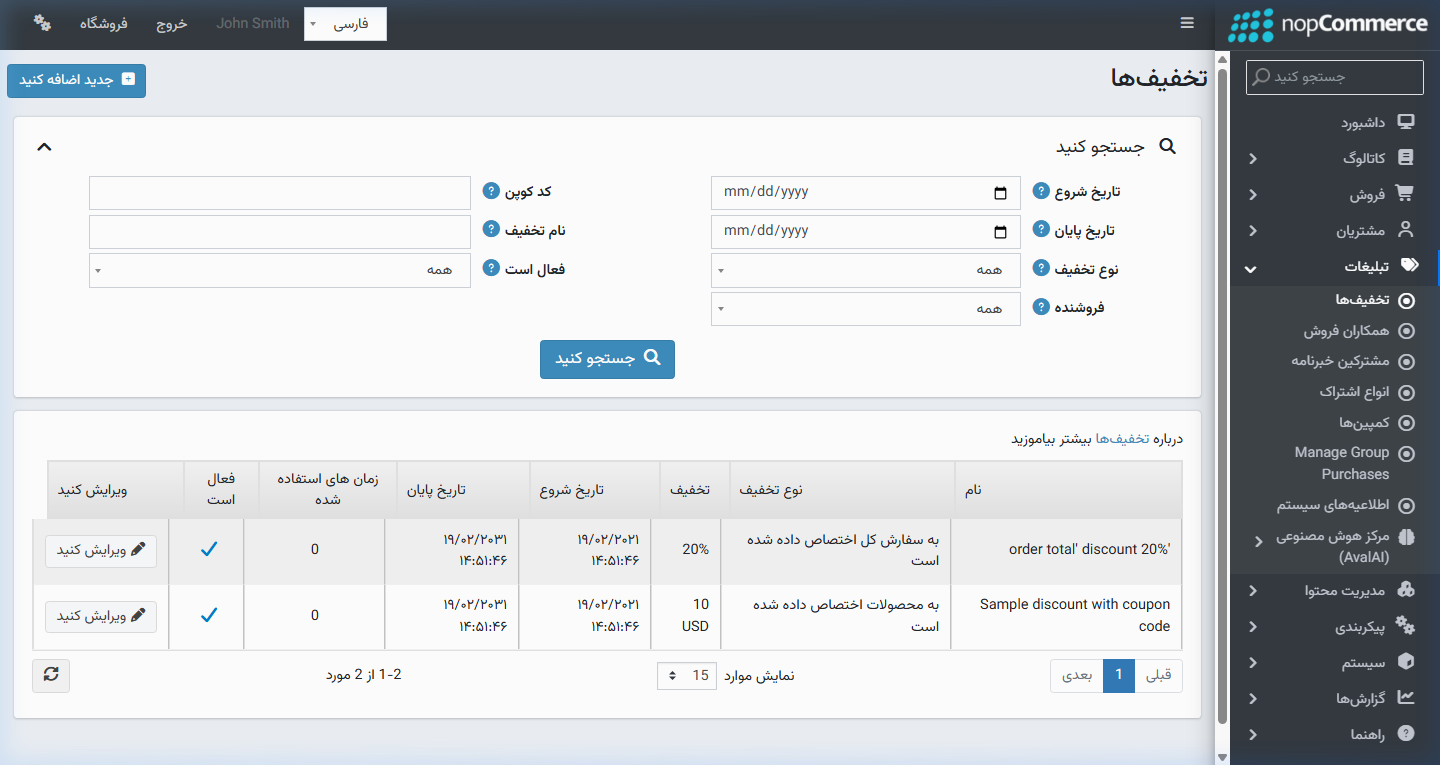
\includegraphics[width=0.85\textwidth]{step1_admin_discounts.png}}
    \caption{گام ۱: مدیریت تخفیف‌ها در پنل ارشد}
    \label{fig:step1_admin_discounts}
\end{figure}

\subsection{گام ۲: مشاهده و خرید از صفحه تخفیف‌ها توسط مشتری}
مشتری به آدرس \url{https://ground-buggy-karaoke.ngrok-free.dev/amazing-discounts} مراجعه نموده و محصولات تخفیف‌دار را مشاهده و خریداری می‌کند.

\begin{figure}[H]
    \centering
    \setlatin{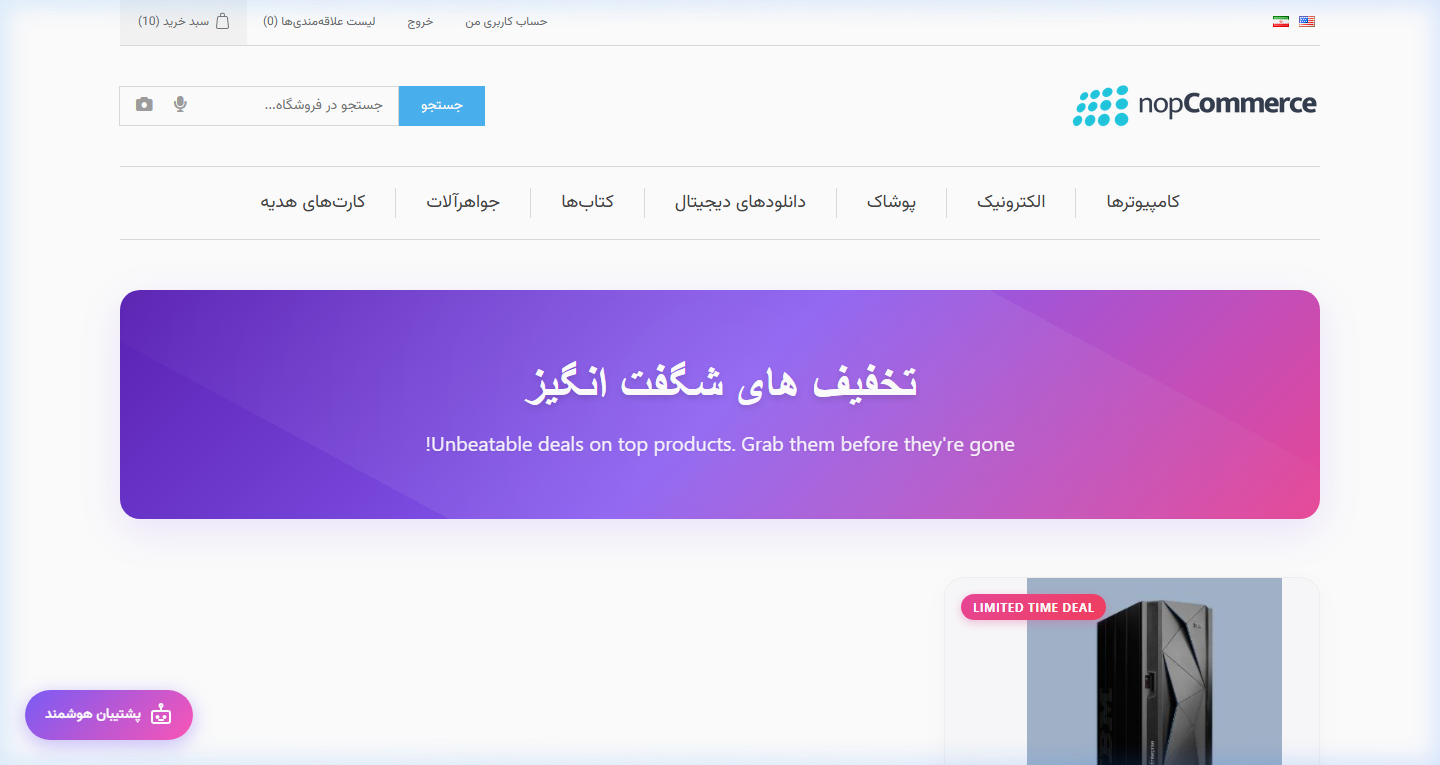
\includegraphics[width=0.85\textwidth]{step2_amazing_discounts.png}}
    \caption{گام ۲: ویترین محصولات تخفیف‌دار در صفحه تخفیف‌های شگفت‌انگیز}
    \label{fig:step2_amazing_discounts}
\end{figure}

\newpage
\section{بخش دوم: راهنمای گام به گام سیستم تبلیغات فروشندگان}

این سیستم به فروشندگان اجازه می‌دهد درخواست برجسته‌سازی و تبلیغ محصولات خود را ثبت کنند.

\subsection{گام ۳: ورود به داشبورد تبلیغات فروشنده (Seller Dashboard)}
فروشنده پس از ورود، به داشبورد تبلیغات خود به آدرس \lr{/seller/dashboard} مراجعه می‌کند.

\begin{figure}[H]
    \centering
    \setlatin{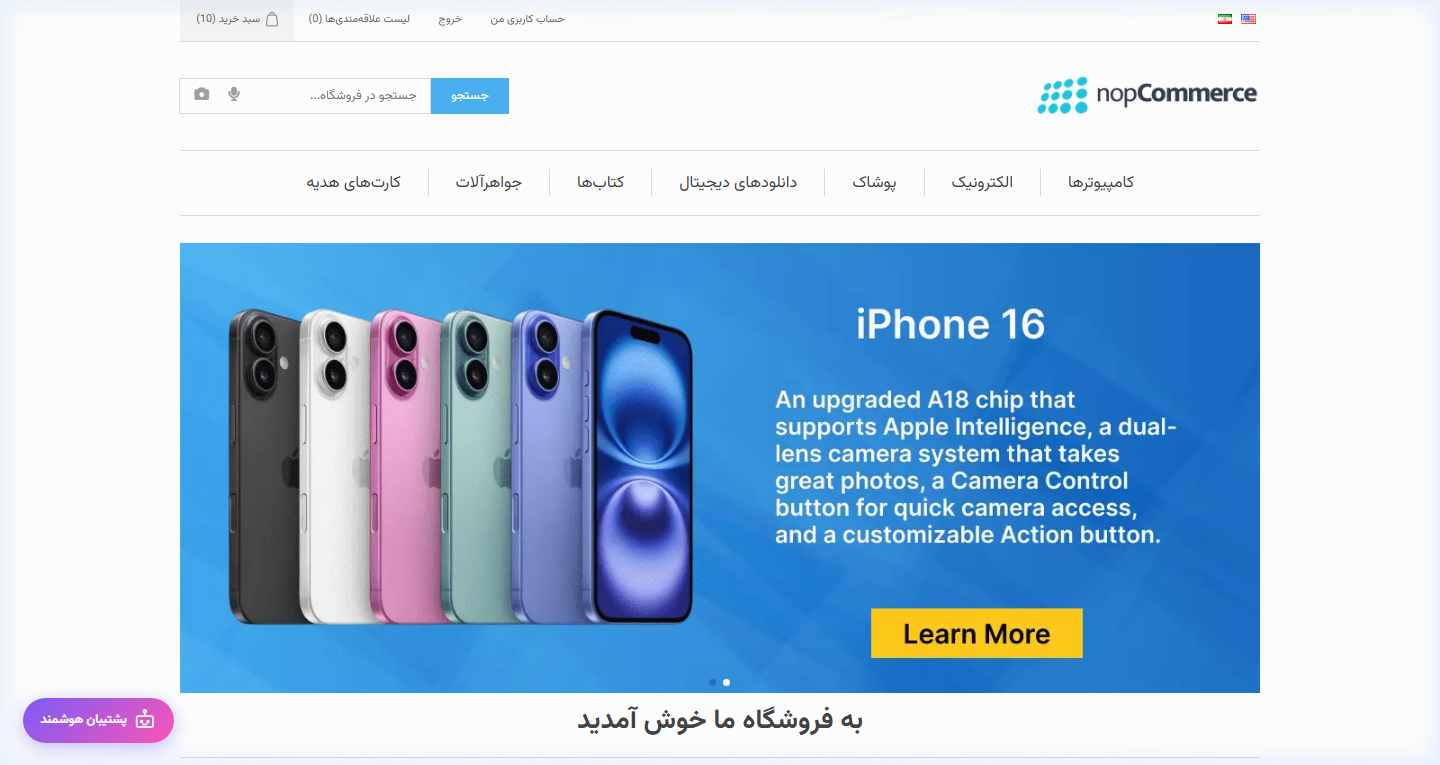
\includegraphics[width=0.85\textwidth]{step3_seller_dashboard.png}}
    \caption{گام ۳: داشبورد تبلیغات و بازاریابی فروشنده}
    \label{fig:step3_seller_dashboard}
\end{figure}

\subsection{گام ۴: ثبت درخواست محصول تبلیغاتی جدید}
فروشنده با کلیک روی دکمه افزودن محصول تبلیغاتی (\lr{/seller/product/add})، فرم ثبت تبلیغ را تکمیل می‌کند.

\begin{figure}[H]
    \centering
    \setlatin{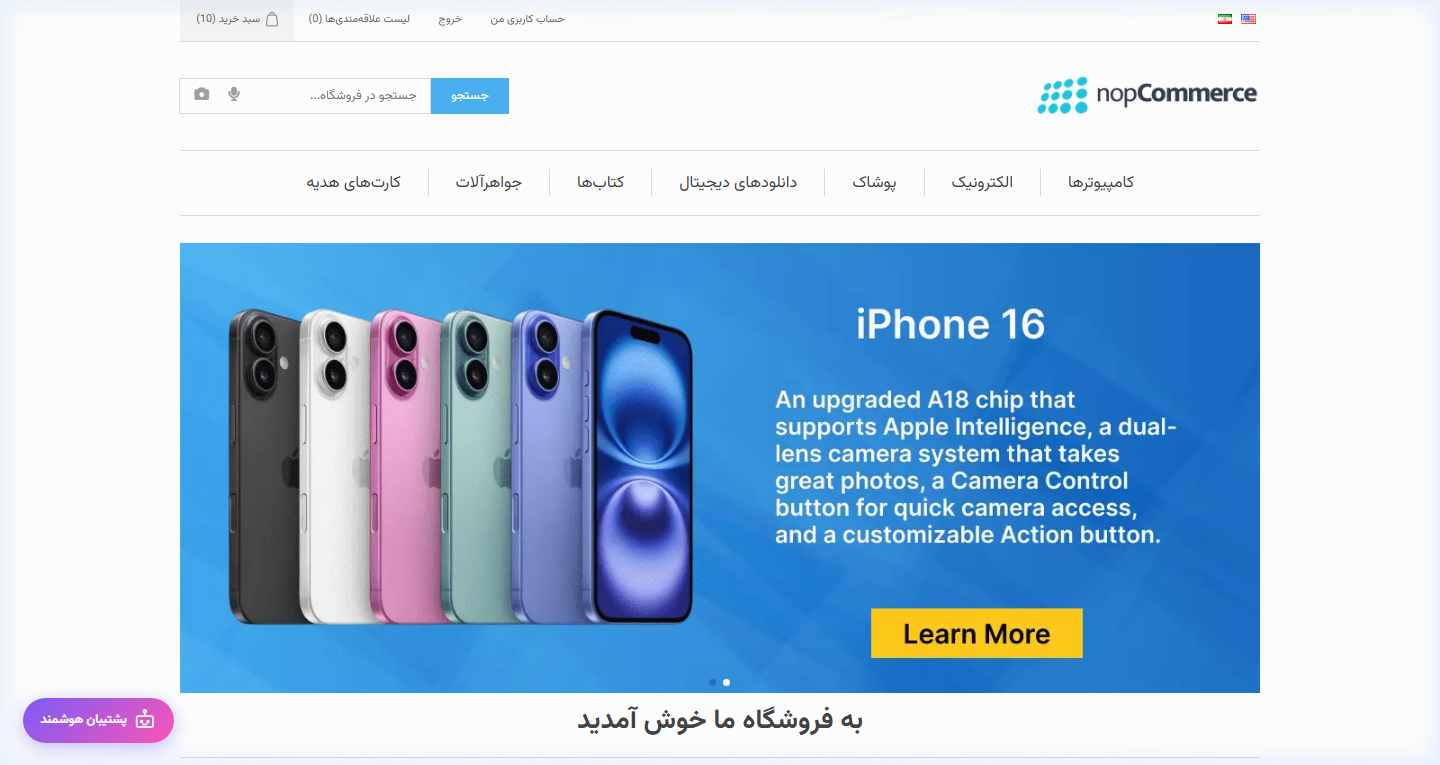
\includegraphics[width=0.85\textwidth]{step4_seller_product_add.png}}
    \caption{گام ۴: فرم ثبت محصول جدید برای تبلیغات}
    \label{fig:step4_seller_product_add}
\end{figure}

\subsection{گام ۵: بررسی و تایید درخواست توسط مدیر (Admin Approval)}
مدیر فروشگاه به مسیر \lr{/Admin/SellerMarketing/List} مراجعه کرده و درخواست‌های تبلیغاتی را بررسی و تایید می‌کند.

\begin{figure}[H]
    \centering
    \setlatin{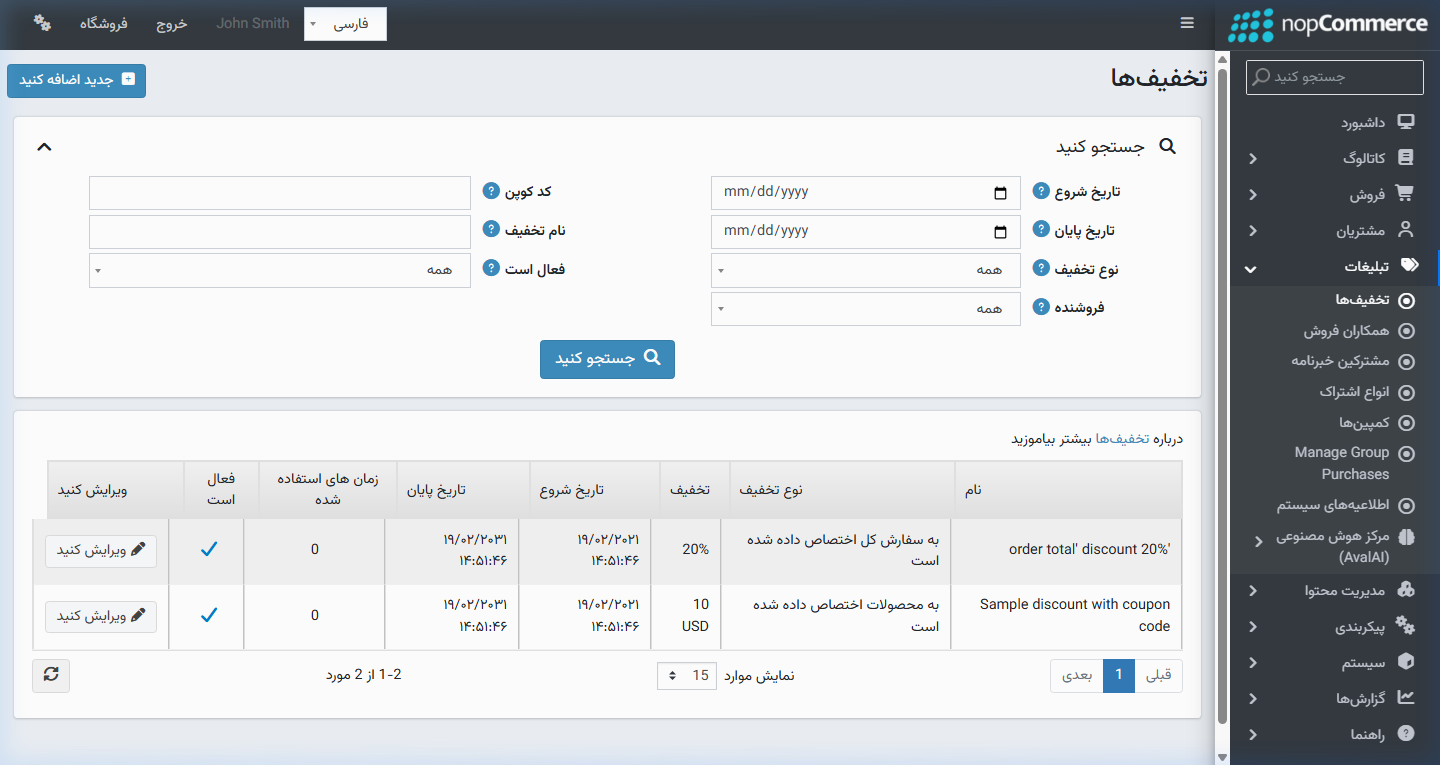
\includegraphics[width=0.85\textwidth]{step5_admin_seller_marketing.png}}
    \caption{گام ۵: مدیریت و تایید درخواست‌های تبلیغاتی فروشندگان در پنل ارشد}
    \label{fig:step5_admin_seller_marketing}
\end{figure}

\newpage
\section{بخش سوم: راهنمای گام به گام سیستم خرید گروهی و کیف پول}

\subsection{گام ۶: فعال‌سازی خرید گروهی محصولات توسط مدیر}
مدیر به مسیر \lr{/Admin/GroupPurchase/List} برمی‌گردد و محصولات را برای خرید گروهی فعال می‌کند.

\begin{figure}[H]
    \centering
    \setlatin{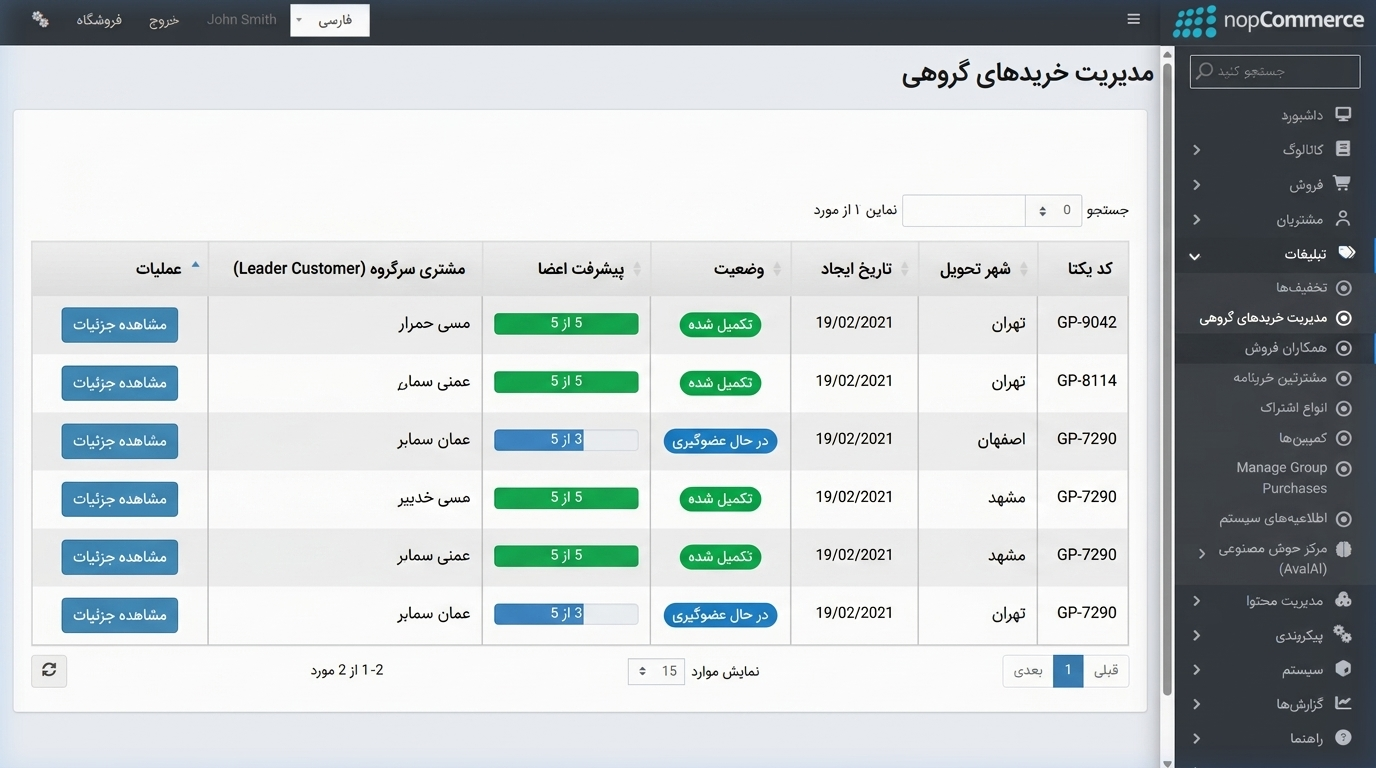
\includegraphics[width=0.85\textwidth]{step6_admin_group_purchase.png}}
    \caption{گام ۶: مدیریت و فعال‌سازی محصولات خرید گروهی}
    \label{fig:step6_admin_group_purchase}
\end{figure}

\subsection{گام ۷: تنظیم قوانین پاداش خرید گروهی توسط مدیر}
مدیر در مسیر \lr{/Admin/RewardRule/List} میزان پاداش واریزی به کیف پول لیدرهای گروه را تعیین می‌کند.

\begin{figure}[H]
    \centering
    \setlatin{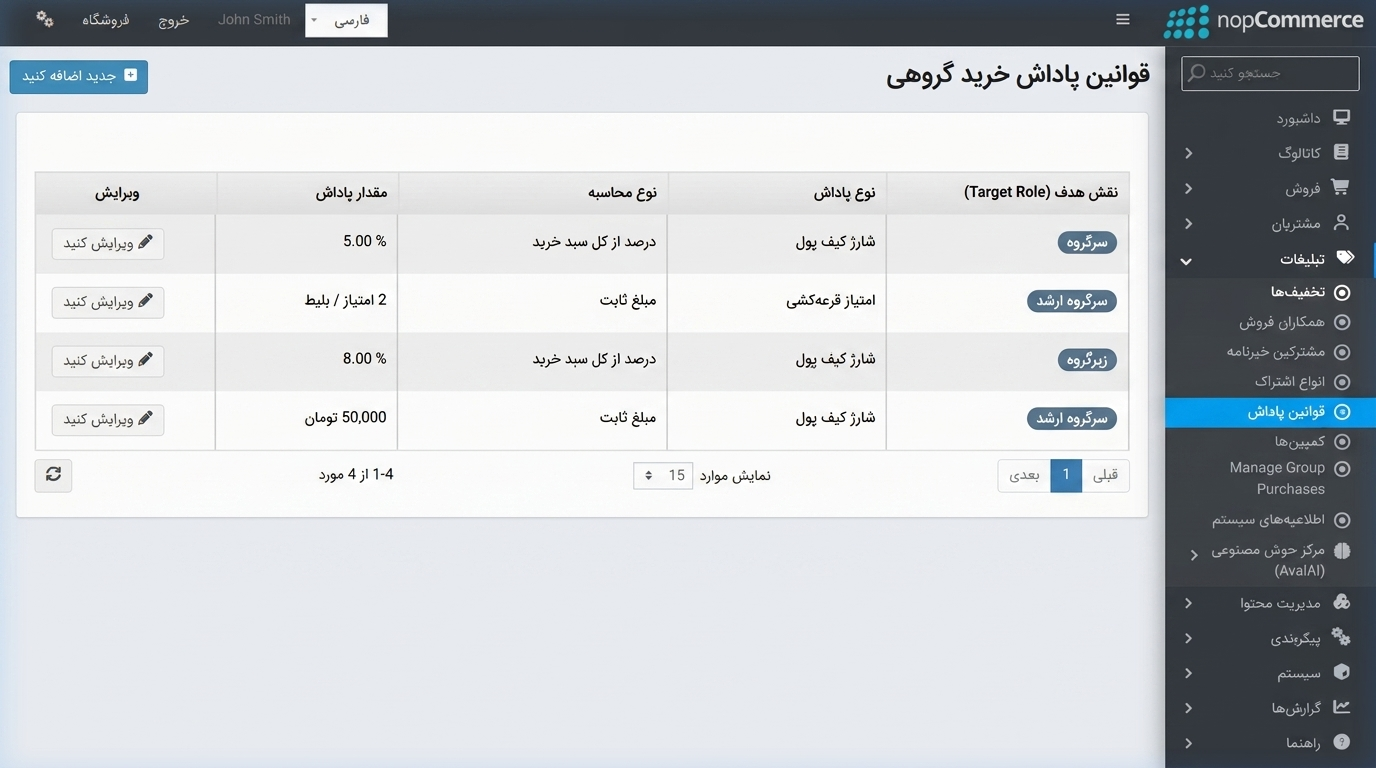
\includegraphics[width=0.85\textwidth]{step7_admin_reward_rules.png}}
    \caption{گام ۷: مدیریت قوانین پاداش خرید گروهی}
    \label{fig:step7_admin_reward_rules}
\end{figure}

\subsection{گام ۸: مدیریت گروه‌های لیدری توسط لیدر}
لیدر می‌تواند وضعیت گروه‌های ایجاد شده خود را در آدرس \lr{/customer/leader-groups} پیگیری نماید.

\begin{figure}[H]
    \centering
    \setlatin{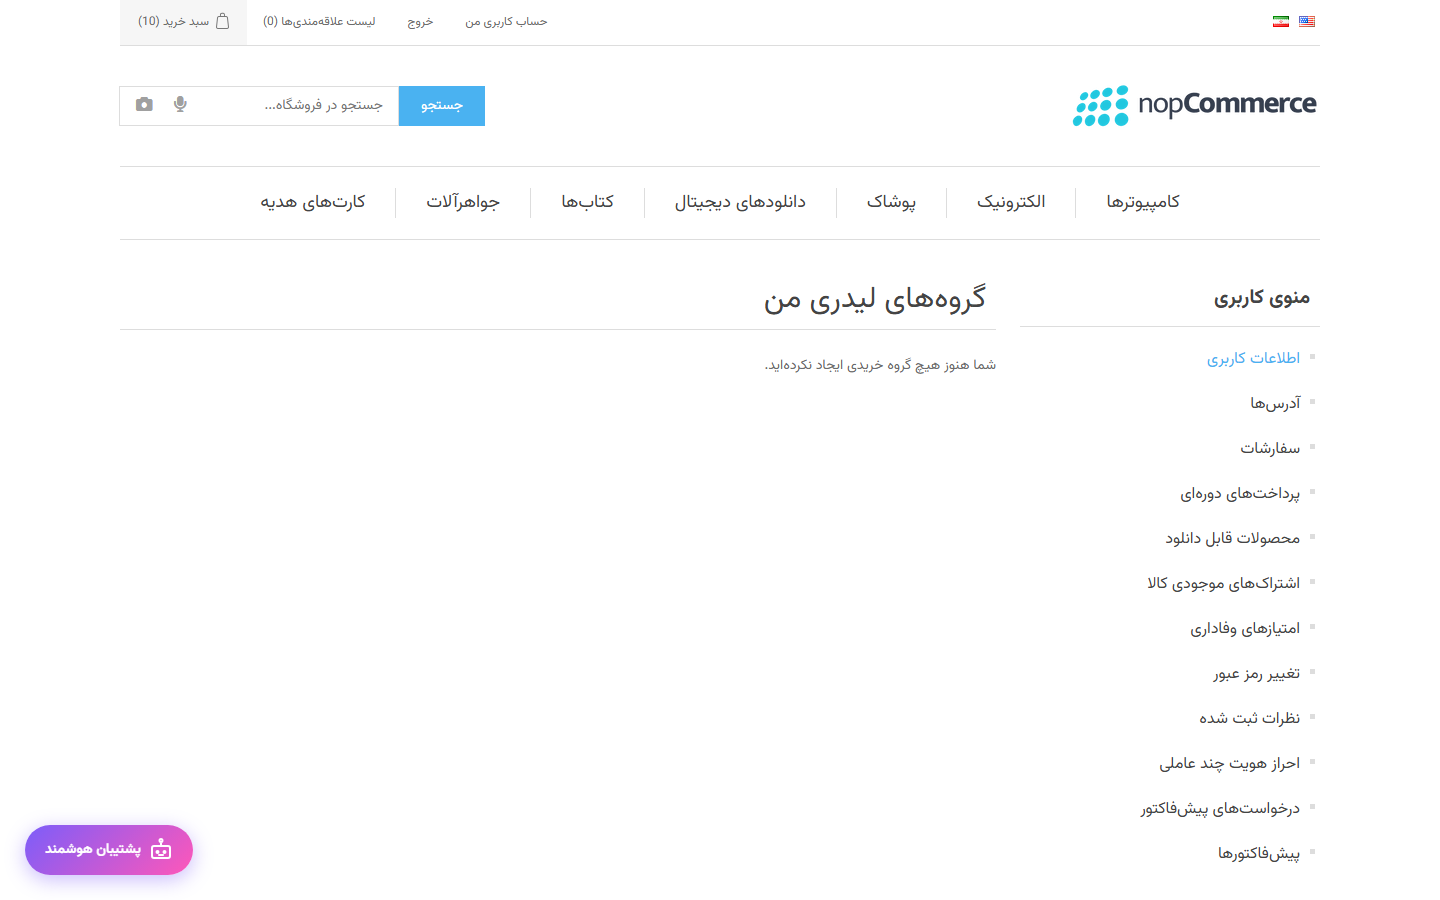
\includegraphics[width=0.85\textwidth]{step8_customer_leader_groups.png}}
    \caption{گام ۸: صفحه گروه‌های لیدری مشتری}
    \label{fig:step8_customer_leader_groups}
\end{figure}

\subsection{گام ۹: مشاهده تاریخچه زیرمجموعه‌ها توسط اعضا}
اعضای گروه‌ها می‌توانند تاریخچه عضویت خود در گروه‌ها را در آدرس \lr{/customer/subgroup-history} مشاهده کنند.

\begin{figure}[H]
    \centering
    \setlatin{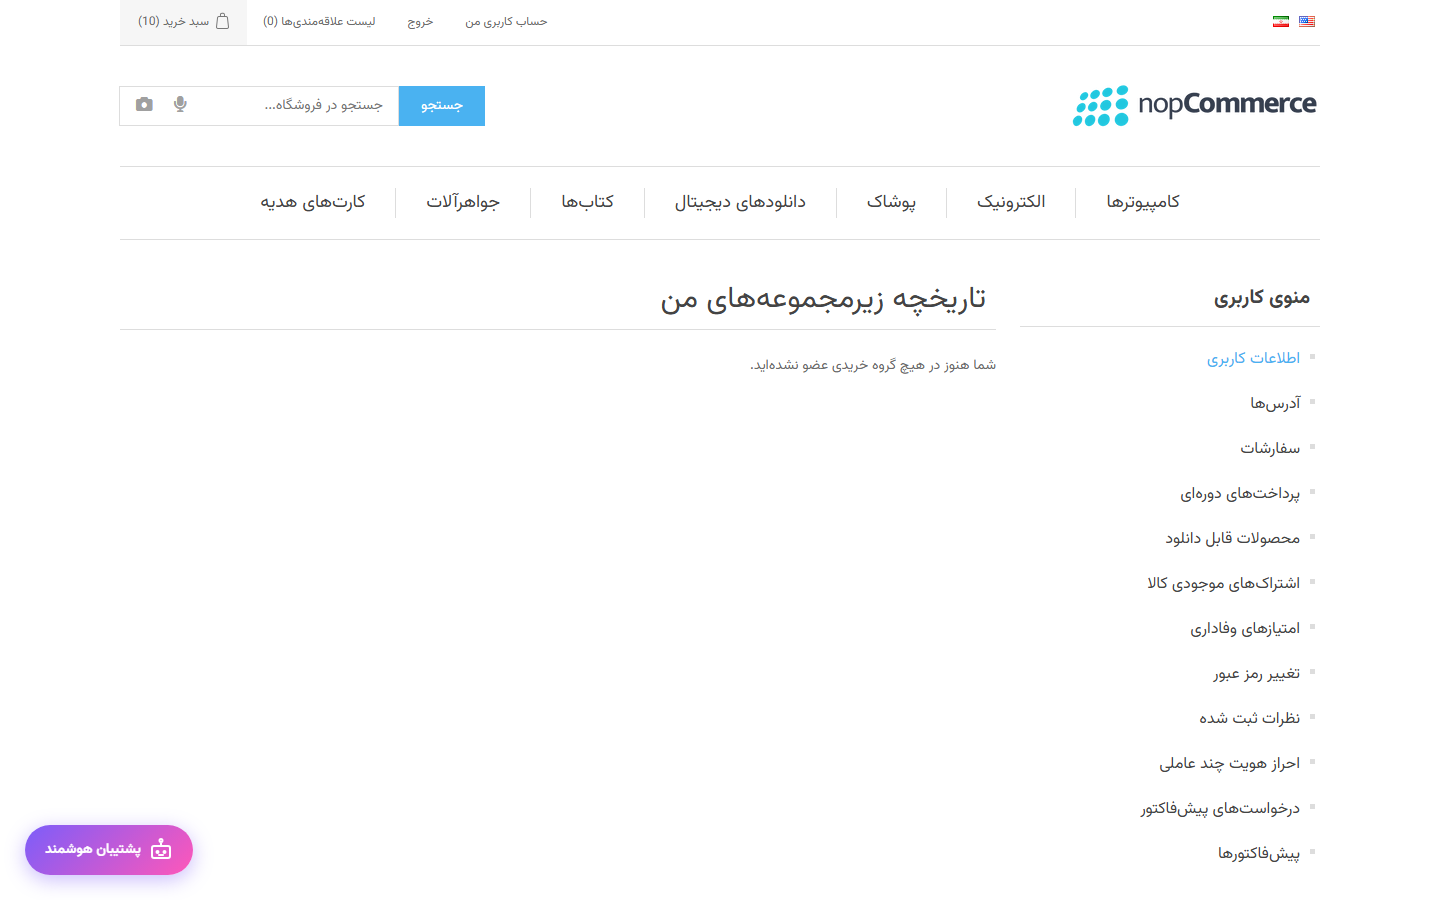
\includegraphics[width=0.85\textwidth]{step9_customer_subgroup_history.png}}
    \caption{گام ۹: تاریخچه زیرمجموعه‌ها و گروه‌های عضو شده}
    \label{fig:step9_customer_subgroup_history}
\end{figure}

\subsection{گام ۱۰: مدیریت کیف پول و موجودی پاداش‌ها}
کاربران موجودی عادی و پاداش خرید گروهی خود را در آدرس \lr{/customer/wallet} مشاهده می‌نمایند.

\begin{figure}[H]
    \centering
    \setlatin{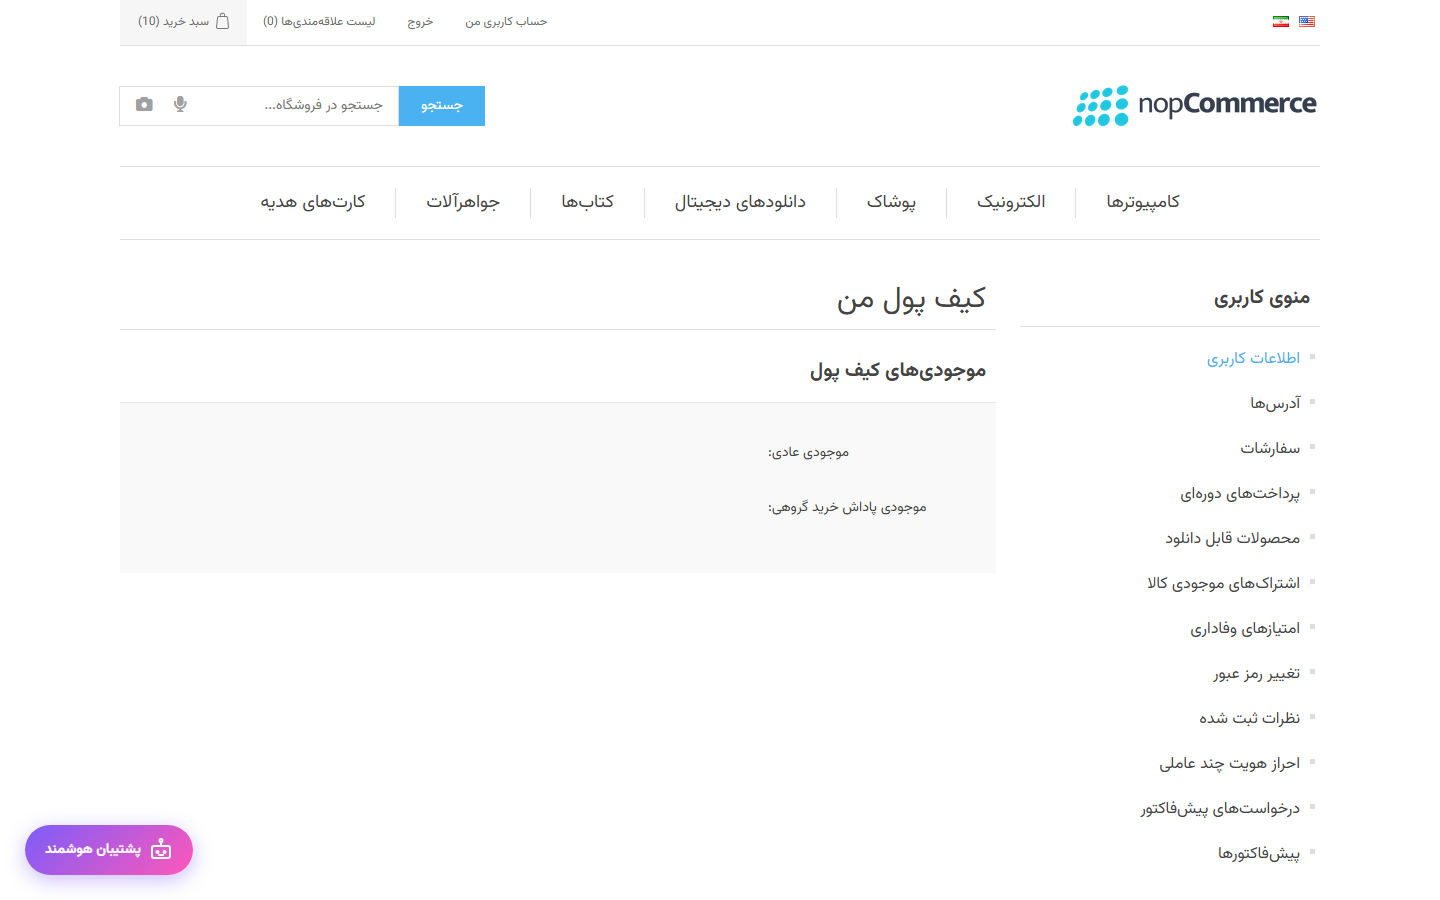
\includegraphics[width=0.85\textwidth]{step10_customer_wallet.png}}
    \caption{گام ۱۰: صفحه کیف پول مشتری و پاداش‌های خرید گروهی}
    \label{fig:step10_customer_wallet}
\end{figure}

\subsection{گام ۱۱: مشاهده امتیازات و شرکت در قرعه‌کشی}
کاربران امتیازات قرعه‌کشی کسب‌شده خود را در آدرس \lr{/customer/lottery} مشاهده و مدیریت می‌کنند.

\begin{figure}[H]
    \centering
    \setlatin{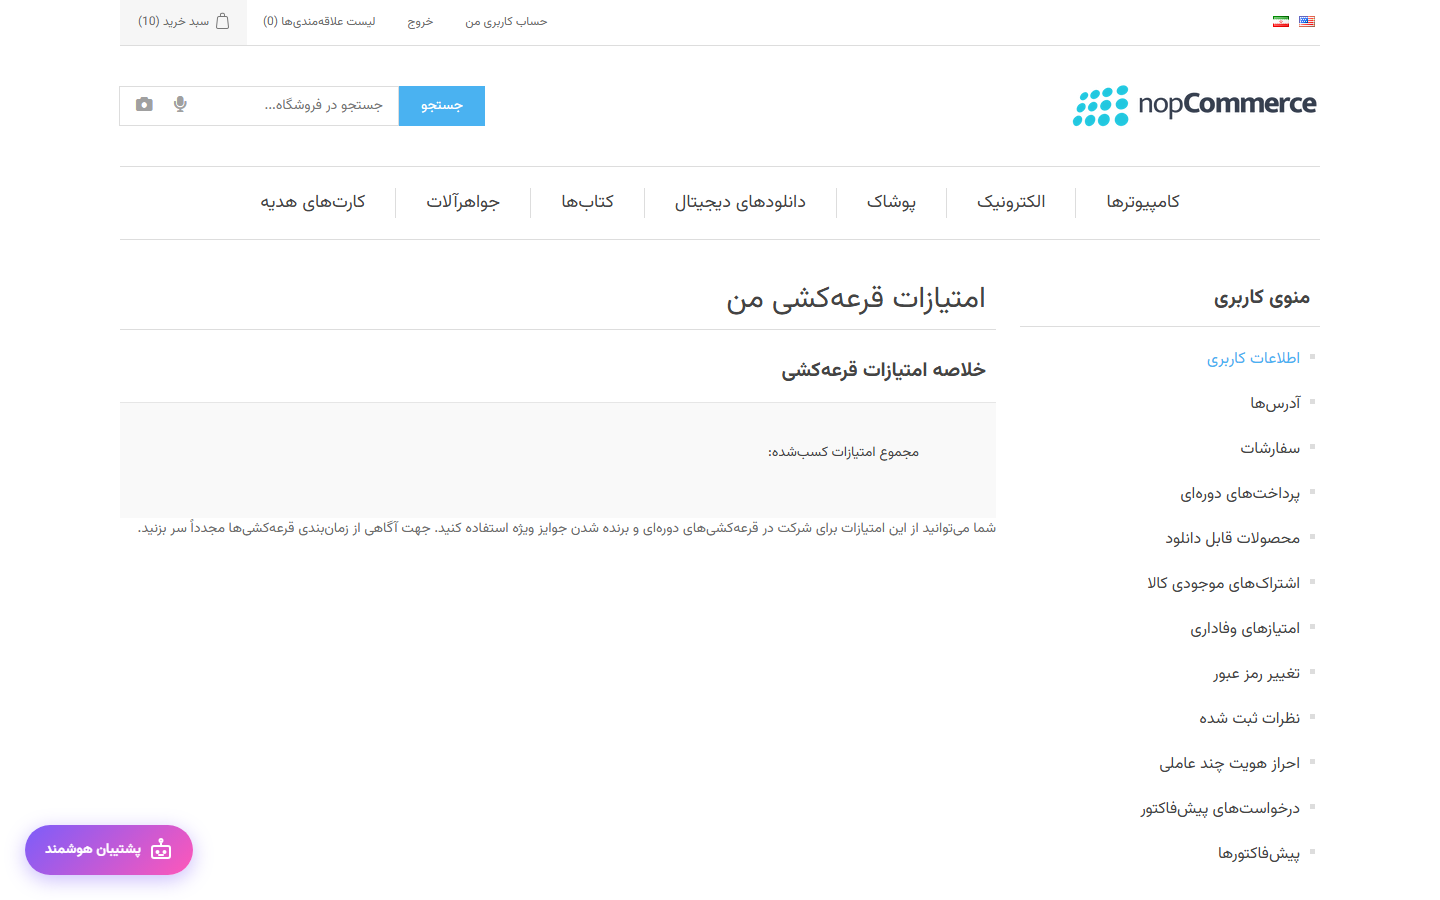
\includegraphics[width=0.85\textwidth]{step11_customer_lottery.png}}
    \caption{گام ۱۱: صفحه امتیازات و قرعه‌کشی مشتری}
    \label{fig:step11_customer_lottery}
\end{figure}

\newpage
\section{بخش چهارم: راهنمای گام به گام ماژول‌های هوشمند (B و C)}

\subsection{گام ۱۲: ماژول B (جستجوی هوشمند - صوتی و تصویری)}
این ماژول قابلیت جستجوی صوتی و تصویری مبتنی بر هوش مصنوعی را در نوار جستجوی عمومی فروشگاه ارائه می‌دهد.

\begin{figure}[H]
    \centering
    \setlatin{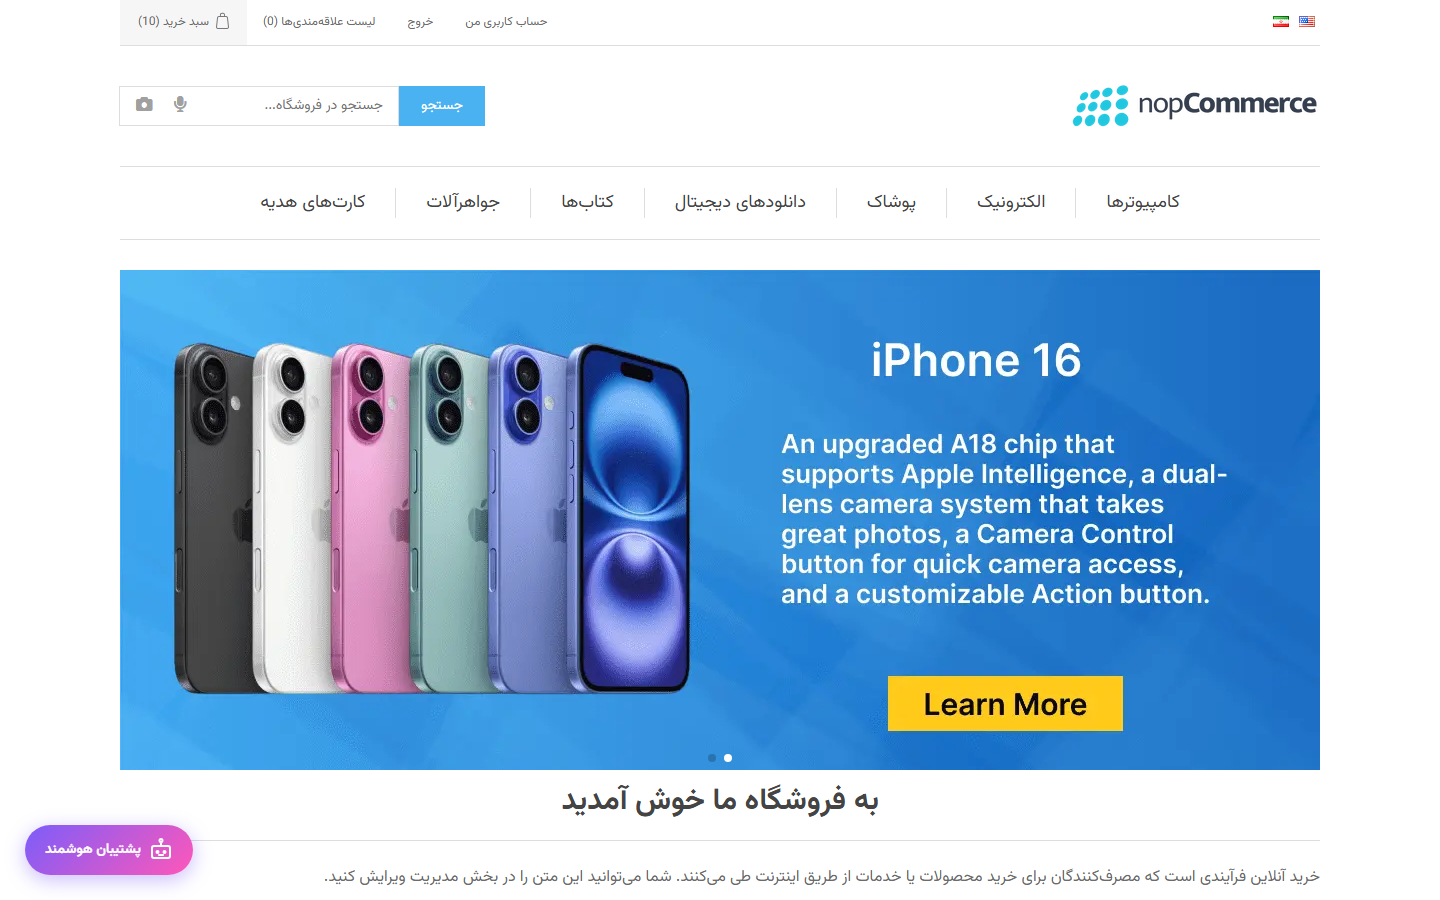
\includegraphics[width=0.85\textwidth]{module_b_smart_search.png}}
    \caption{گام ۱۲: ماژول جستجوی هوشمند (جستجوی صوتی و تصویری هوش مصنوعی)}
    \label{fig:module_b_smart_search}
\end{figure}

\subsection{گام ۱۳: ماژول C (تشخیص محصولات تکراری با هوش مصنوعی)}
این ماژول محصولات ثبت شده توسط فروشندگان را به صورت خودکار تحلیل کرده و از ثبت کالای تکراری در انبارداری جلوگیری می‌نماید.

\begin{figure}[H]
    \centering
    \setlatin{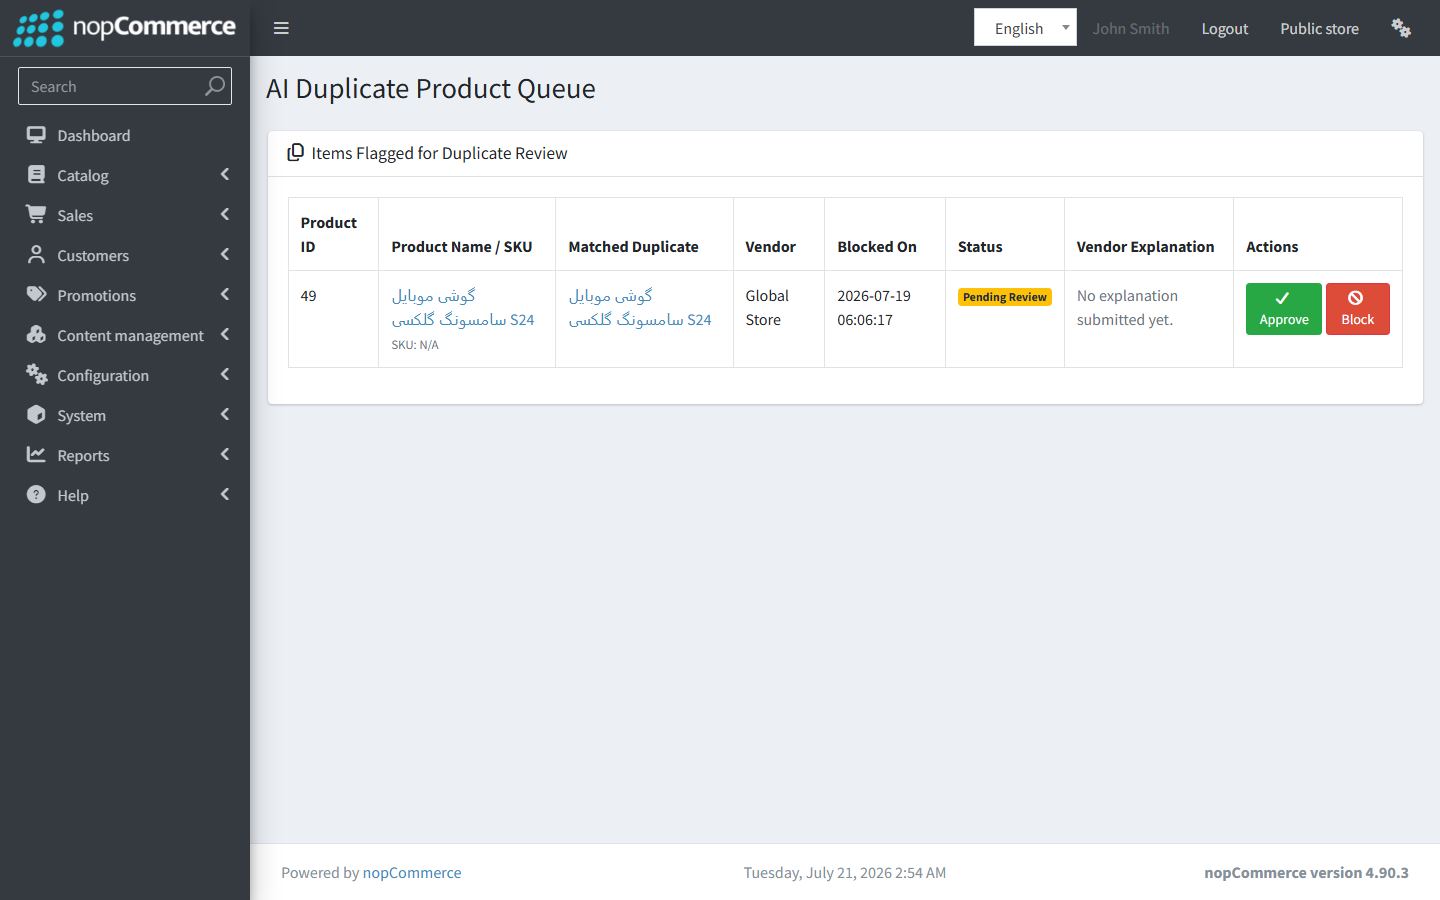
\includegraphics[width=0.85\textwidth]{module_c_duplicate_detection.png}}
    \caption{گام ۱۳: ماژول تشخیص محصولات تکراری با هوش مصنوعی در پنل ارشد}
    \label{fig:module_c_duplicate_detection}
\end{figure}

\newpage
\section{جدول مرجع آدرس‌های سیستم (فروشگاه و مدیریت)}

\begin{table}[H]
\centering
\caption{جدول کامل مسیرهای دسترسی به همراه شماره گام}
\vspace{0.3cm}
\begin{tabular}{p{2cm} p{4.5cm} p{5.5cm} p{4.5cm}}
\toprule
\textbf{شماره گام} & \textbf{نام بخش / قابلیت} & \textbf{آدرس بخش فروشگاه} & \textbf{آدرس بخش مدیریت} \\
\midrule
گام ۱ & مدیریت تخفیف‌ها & --- & \lr{/Admin/Discount/List} \\
گام ۲ & صفحه تخفیف‌های شگفت‌انگیز & \lr{/amazing-discounts} & --- \\
گام ۳ & داشبورد تبلیغات فروشنده & \lr{/seller/dashboard} & --- \\
گام ۴ & ثبت محصول تبلیغاتی & \lr{/seller/product/add} & --- \\
گام ۵ & مدیریت تبلیغات فروشندگان & --- & \lr{/Admin/SellerMarketing/List} \\
گام ۶ & مدیریت خرید گروهی & --- & \lr{/Admin/GroupPurchase/List} \\
گام ۷ & مدیریت قوانین پاداش & --- & \lr{/Admin/RewardRule/List} \\
گام ۸ & گروه‌های لیدری مشتری & \lr{/customer/leader-groups} & --- \\
گام ۹ & تاریخچه زیرمجموعه‌ها & \lr{/customer/subgroup-history} & --- \\
گام ۱۰ & کیف پول و موجودی & \lr{/customer/wallet} & \lr{/Admin/CustomerWallet/List} \\
گام ۱۱ & امتیازات و قرعه‌کشی & \lr{/customer/lottery} & --- \\
گام ۱۲ & ماژول جستجوی هوشمند & \lr{/AiSearch/VisualSearch} & --- \\
گام ۱۳ & ماژول تشخیص تکراری & --- & \lr{/Admin/AiDuplicateProduct/List} \\
\bottomrule
\end{tabular}
\end{table}

\end{document}
